\documentclass{article}
\usepackage[utf8]{inputenc}
\usepackage[T1]{fontenc}
\usepackage[english]{babel}
\usepackage{graphicx}
\usepackage{physics}
\usepackage{calrsfs}
\usepackage{mathalpha}
\usepackage{amssymb}
\usepackage{amsfonts}
\usepackage{amsmath}
\usepackage{fixltx2e}
\usepackage[dvipsnames]{xcolor}

\definecolor{myDarkGreen}{RGB}{0, 128, 0}


\title{2021-03-16 theory}
\author{}
\date{March 2021}

\begin{document}


\maketitle

\section{Key exchange protocol}
Key exchange (also key establishment) is a method in cryptography by which cryptographic keys are exchanged between two parties, allowing use of a cryptographic algorithm. The key exchange problem describes ways to exchange whatever keys or other information are needed for establishing a secure communication channel so that no one else can obtain a copy. Historically, before the invention of public-key cryptography (asymmetrical cryptography), symmetric-key cryptography utilized a single key to encrypt and decrypt messages. For two parties to communicate confidentially, they must first exchange the secret key so that each party is able to encrypt messages before sending, and decrypt received ones. This process is known as the key exchange.


\subsection{Diffie–Hellman key exchange}
In 1976, Whitfield Diffie and Martin Hellman published a cryptographic protocol called the Diffie–Hellman key exchange (D–H) based on concepts developed by Hellman's PhD student Ralph Merkle. The protocol enables users to securely exchange secret keys even if an opponent is monitoring that communication channel. The D–H key exchange protocol, however, does not by itself address authentication (i.e. the problem of being sure of the actual identity of the person or 'entity' at the other end of the communication channel).
\begin{figure}[htb]
	\begin{center}
  		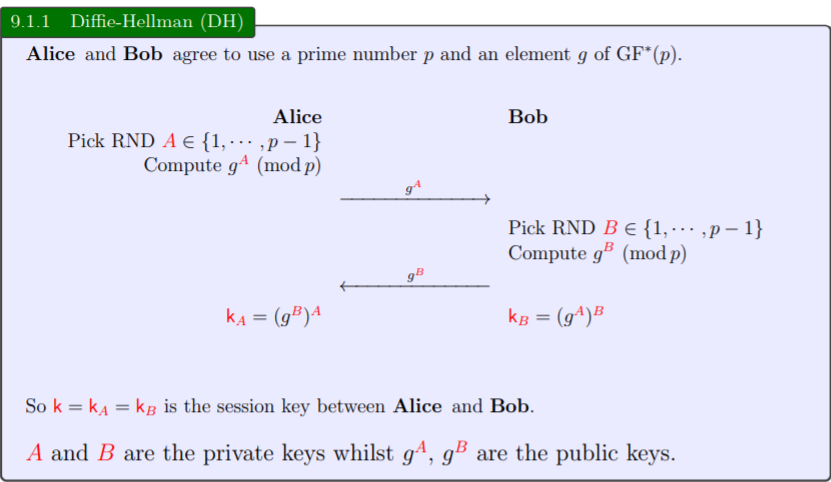
\includegraphics[width=1 \textwidth,]{Diffie-Hellman.png}
 	\end{center}
 	\caption{In the Diffie–Hellman key exchange scheme, each party generates a public/private key pair and distributes the public key. After obtaining an authentic copy of each other's public keys, Alice and Bob can compute a shared secret offline. The shared secret can be used, for instance, as the key for a symmetric cipher.}
 	\label{ciphering}
\end{figure}
\newpage
\subsubsection{Behaviour}
The simplest and the original implementation of the protocol uses the multiplicative group of integers modulo p, where p is prime, and g is a primitive root modulo p. These two values are chosen in this way to ensure that the resulting shared \textbf{secret} can take on any value from 1 to p–1. Here is an example of the protocol, with non-secret values in \textit{italics}, and secret values in \textbf{bold}.
\subsubsection{Exercise 9.1.1}

\begin{enumerate}
\item Alice and Bob publicly agree to use a modulus \textit{p} = 23 and base \textit{g} = 5 (which is a primitive root modulo 23).
\item Alice chooses a secret integer \textbf{a} = 4, then sends Bob A = $\textit{g}^\textbf{a} \mod\textit{ p}$

\begin{itemize}
\item \textit{A} =$ \textit{5}^\textbf{4} \mod \textit{23}$ = \textit{4}

\end{itemize}
\item Bob chooses a secret integer \textbf{b} = 3, then sends Alice B = $\textit{g}^\textbf{b} \mod \textit{p}$
\begin{itemize}
\item \textit{B} =$ \textit{5}^\textbf{3} \mod \textit{23}$ = \textit{10}
\end{itemize}
\item Alice computes \textbf{s} = $\textit{B}^\textbf{a} \mod \textit{p}$
\begin{itemize}
\item \textbf{s} = $\textit{10}^\textbf{4} \mod \textit{23}$ = \textbf{18}
\end{itemize}
\item Bob computes \textbf{s} = $\textit{A}^\textbf{b} \mod \textit{p}$
\begin{itemize}
\item \textbf{s} =  $\textit{4}^\textbf{3}  \mod \textit{23}$ = \textbf{18}
\end{itemize}
\item Alice and Bob now share a secret (the number 18).\\

In applications p should have at least 2048 bits to avoid attacks as index calculus. More info
here: https://www.keylength.com/en/compare/

Both Alice and Bob have arrived at the same values because under $\mod p$ :$ {\displaystyle {\color {Blue}A }^{\color {Red}b}{\bmod {\color {Blue}p}}={\color {Blue}g}^{\color {Red}ab}{\bmod {\color {Blue}p}}={\color {Blue}g}^{\color {Red}ba}{\bmod {\color {Blue}p}}={\color {Blue}B}^{\color {Red}a}{\bmod {\color {Blue}p}}}$\\ More specifically : ${\displaystyle ({\color {Blue}g}^{\color {Red}a}{\bmod {\color {Blue}p}})^{\color {Red}b}{\bmod {\color {Blue}p}}=({\color {Blue}g}^{\color {Red}b}{\bmod {\color {Blue}p}})^{\color {Red}a}{\bmod {\color {Blue}p}}}$\\

\subsubsection{Man in the Middle (MITM)}
In the original description, the Diffie–Hellman exchange by itself does not provide authentication of the communicating parties and is thus vulnerable to a man-in-the-middle attack. Oscar (an active attacker executing the man-in-the-middle attack) may establish two distinct key exchanges, one with Alice and the other with Bob, effectively masquerading as Alice to Bob, and vice versa, allowing her to decrypt, then re-encrypt, the messages passed between them. Note that Oscar must continue to be in the middle, actively decrypting and re-encrypting messages every time Alice and Bob communicate. If she is ever absent, her previous presence is then revealed to Alice and Bob. They will know that all of their private conversations had been intercepted and decoded by someone in the channel. In most cases it will not help them get Oscar's private key, even if she used the same key for both exchanges.

A method to authenticate the communicating parties to each other is generally needed to prevent this type of attack. Variants of Diffie–Hellman, such as STS protocol, may be used instead to avoid these types of attacks.
\begin{figure}[htb]
	\begin{center}
  		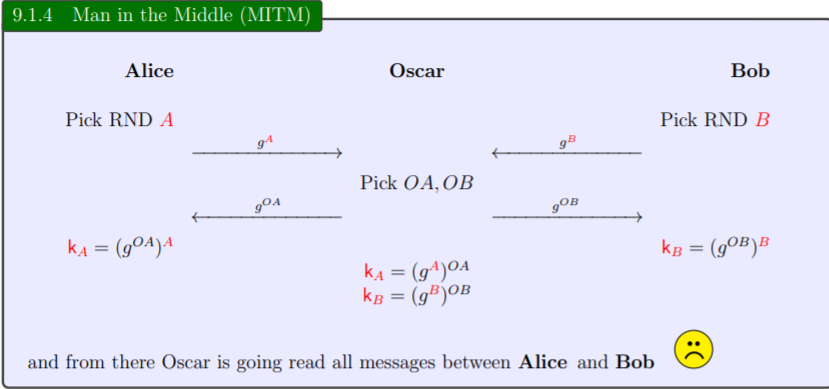
\includegraphics[width=1 \textwidth]{MITM.png}
 	\end{center}
 	\caption{}
 	\label{ciphering}
\end{figure}





\end{enumerate}
\newpage




\section{Public Key Encryption}
Public-key cryptography, or asymmetric cryptography, is a cryptographic system that uses pairs of keys: public keys (which may be known to others), and private keys (which may never be known by any except the owner). The generation of such key pairs depends on cryptographic algorithms which are based on mathematical problems termed one-way functions. Effective security requires keeping the private key private; the public key can be openly distributed without compromising security.
\begin{figure}[htb]
	\begin{center}
  		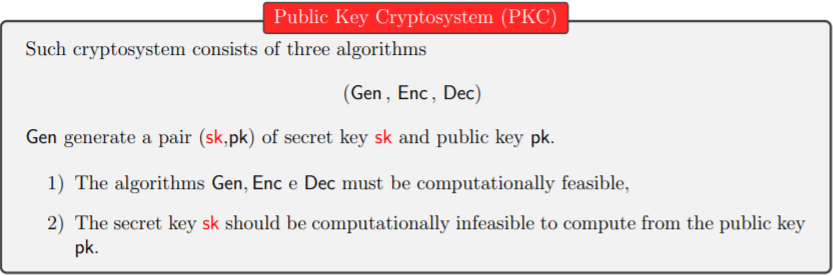
\includegraphics[width=1 \textwidth]{PublicKeyCrypto.png}
 	\end{center}
 	\caption{An unpredictable (typically large and random) number is used to begin generation of an acceptable pair of keys suitable for use by an asymmetric key algorithm.}
 	\label{ciphering}
\end{figure}
\subsection{ElGamal}
In cryptography, the ElGamal encryption system is an asymmetric key encryption algorithm for public-key cryptography which is based on the Diffie–Hellman key exchange. It was described by Taher Elgamal in 1985. ElGamal encryption is used in the free GNU Privacy Guard software, recent versions of PGP, and other cryptosystems. ElGamal system is based on the difficulty of discrete logarithm problem where it is directly forward to raise numbers to large powers but it is much harder to do the inverse computation of the discrete logarithm. \\
\textbf{The discrete logarithm:} When dealing with real numbers, then the solution of the equation y=$b^x$ can be found such that x= $log_b y $. Given the integers b and n such that b<n, the discrete logarithm of integer y to the base b is an integer x, such that $b^x=y \mod n$. Hence, unlike logarithms, the discrete logarithm problem is defined in a discrete domain where a solution must be exact.
\subsubsection{Algorithm}
The ElGamal encryption system parameters consists of a prime number (p) and an integer number (g) which is a root of (p-1) and whose power modulo (p) generate a large number of elements.
\begin{align*}
  \intertext{To encrypt plaintext, a private key (a) is used to generate the public key (y) as given in such that (a) is an integer between 1 and p-2.} 
  {y = g ^ a \mod p};\\ \intertext{The public key for ElGamal encryption algorithm consists of the triple (p,g,y).\\To encrypt a plaintext message (m), a random integer (k) is chosen such that it is between 1 and p-2. The message is converted to numbers before producing the ciphertext (c) which consists of the pair (y1,y2) calculated as given by and b;} 
  {y1= g^k \mod p };\\
  {y2 = m y^k \mod p};\\ \intertext{The decryption process is applied in a reverse order such that the encrypted message (y1,y2) is used with the private key (a ) and the prime number (p) to retrieve the original message (m) as given;}\\
  {m =\frac{y2}{y1^a} \mod p}; \\ \intertext{The division by $y1^a$ in the last equation should be interpreted in the context of modular arithmetic, that is y2 is multiplied by the inverse of $y1^a$.}
\end{align*}

In a practical setting, ElGamal encryption does not really give a benefit when using it as an encryption scheme as it is, since it does only support message of size of elements of the group being used and parameters must be chosen carefully in order to obtain IND-CPA security (holds always in elliptic curves but you have to choose a suitable subgroup of $\mathbb{Z}_p^*$ to obtain it).  ElGamal encryption, when the paramters are chosen in the right way achieves the weaker notion of indistinguishability under chosen plaintext attacks (IND-CPA). \\

Security of the ElGamal algorithm depends on the (presumed) difficulty of computing discrete logs in a large prime modulus.
\begin{itemize}
\item ElGamal has the disadvantage that the ciphertext is twice  as long as the plaintext. 
\item It has the advantage the same plaintext gives a different ciphertext (with near certainty) each time it is encrypted
\end{itemize}

\subsection{Rabin cryptosystem}
Rabin Cryptosystem is an public-key cryptosystem invented by Michael Rabin. It uses asymmetric key encryption for communicating between two parties and encrypting the message. The security of Rabin cryptosystem is related to the difficulty of factorization. It has the advantage over the others that the problem on which it banks has proved to be hard as integer factorization. It has the disadvantage also, that each output of the Rabin function can be generated by any of four possible inputs. if each output is a ciphertext, extra complexity is required on decryption to identify which of the four possible inputs was the true plaintext.
\subsubsection{Encryption Algorithm}
Like all asymmetric cryptosystems, the Rabin system uses a key pair: a public key for encryption and a private key for decryption. The public key is published for anyone to use, while the private key remains known only to the recipient of the message.\\

\textbf{Key generation}\\
The keys for the Rabin cryptosystem are generated as follows:
\begin{enumerate}
\item Choose two large distinct prime numbers \textbf{p} and \textbf{q} such that \textbf{p }$ \equiv 3 \mod 4  and \textbf{q } \equiv 3\mod 4$
\item Compute \textbf{n}=pq.
\end{enumerate}
Then \textbf{n} is the public key and the pair (p,q) is the private key.\\

\textbf{Encryption}\\
A message M can be encrypted by first converting it to a number $m<n$ using a reversible mapping, then computing $c = m^2 \mod n$. The ciphertext is c.\\

\textbf{Decryption}\\
The message m can be recovered from the ciphertext c by taking its square root modulo n as follows.
\begin{enumerate}
\item Compute the square root of c modulo p and q using these formulas:
\begin{align*}
    {m_p=c^\frac{1(p+1)}{4} \mod p}\\
    {m_q=c^\frac{1(q+1)}{4} \mod q}
\end{align*}
\item Use the extended Euclidean algorithm to find $y_{p}$ and $y_{q}$ such that ${\displaystyle y_{p}\cdot p+y_{q}\cdot q=1}y_{p}\cdot p+y_{q}\cdot q=1$.
\item Use the Chinese remainder theorem to find the four square roots of c modulo n:

 \begin{align*}r_{1}&=\left(y_{p}\cdot p\cdot m_{q}+y_{q}\cdot q\cdot m_{p}\right){\bmod {n}}\\r_{2}&=n-r_{1}\\r_{3}&=\left(y_{p}\cdot p\cdot m_{q}-y_{q}\cdot q\cdot m_{p}\right){\bmod {n}}\\r_{4}&=n-r_{3}\end{align*}
\end{enumerate}
One of these four values is the original plaintext m, although which of the four is the correct one cannot be determined without additional information.
\begin{figure}[htb]
	\begin{center}
  		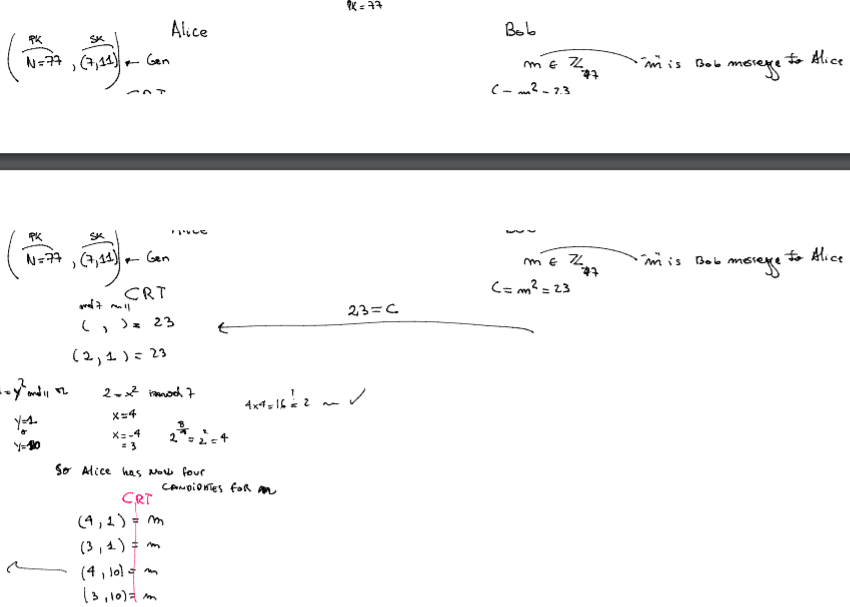
\includegraphics[width=1 \textwidth]{exercise9.2.7.png}
 	\end{center}
 	\caption{Exercise 9.2.7}
 	\label{ciphering}
\end{figure}








\end{document}
